%--------------------------------- Constraints - Preface -------------------------------------------------------
\subsubsection{Technology Leader Constraints and DCC Constraints}
\label{sec:TVA:constraints}
\begin{figure}
    \centering
    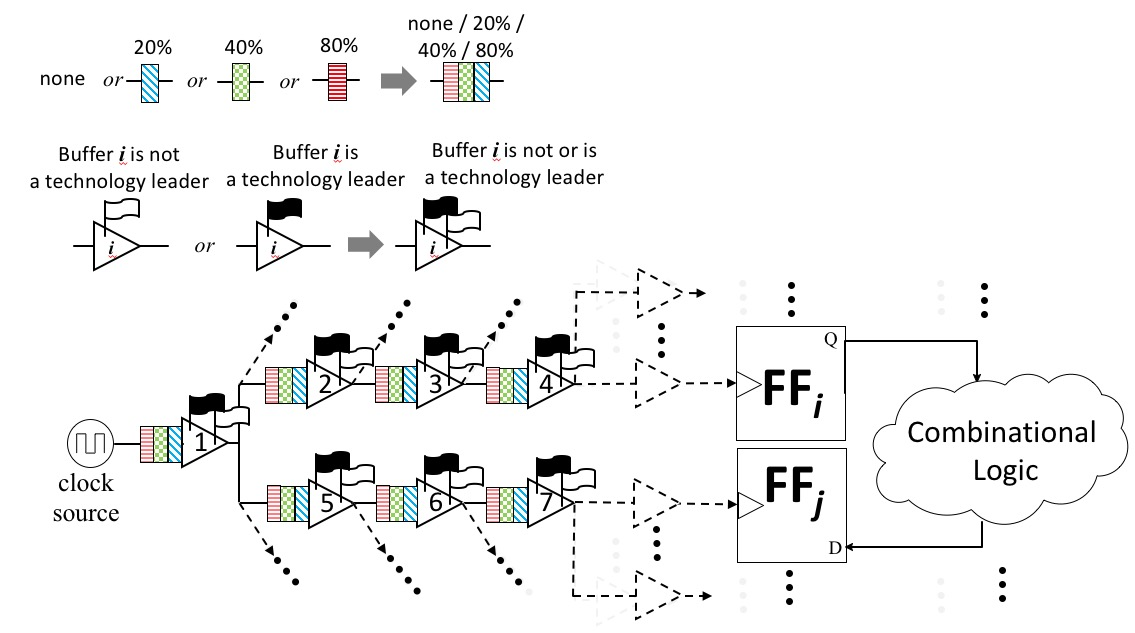
\includegraphics[width=1\columnwidth]{All_types_of_DCCs_and_leaders.png}
    \caption{Generalized DCC insertion and technology leader selection for a target pair of flip-flops}
    \label{fig:g_dcc_leader}
\end{figure}

Figure~\ref{fig:g_dcc_leader} shows a generalized example of DCC insertion and technology leader selection for a pair of flip-flops (\ce{FF_i} and \ce{FF_j}), where there exist aging-critical paths from \ce{FF_i} to \ce{FF_j}. As described in Section~\ref{subsec:dccccc}, a path is defined as an aging-critical path if it is possible to determine the clock period of the circuit, in the presence of aging. Each pair of flip-flops between which there exist aging-critical paths needs to be considered. Here, we use the generalized example to illustrate our SAT-based formulation. The generalized example in Figure~\ref{fig:g_dcc_leader} is similar to that in Figure~\ref{fig:dcctype}. In contrast, we include technology leader selection for each clock buffer in Figure~\ref{fig:g_dcc_leader}. Moreover, we can find that, if the clock buffer, which is selected as a technology leader, is deep in the clock tree (i.e., close to flip-flops), the count of V\textsubscript{th}-reassigned buffers decreases thus the impact of tech-induced clock skew becomes insignificant. The above phenomenon is similar to that in Section ~\ref{subsec:eddcd}, which observes that deeper DCC deployment causes less aging-induced clock skew. Thus, we set a rule of avoiding selecting/inserting leaders/DCCs at a clock tree level, which is larger/deeper than a specified boundary.  The rule greatly reduce the complexity of SAT-based formulation, because a significant fraction of buffers are not considered being inserted DCC at their inputs and being selected as a technology leader. For instance, in Figure~\ref{fig:g_dcc_leader}, dashed buffers and their downstream buffers are not considered. 

In Figure~\ref{fig:g_dcc_leader}, buffers 1 - 7 are candidate locations for DCC insertion and leader selection. According to the encoding mechanism explained in Section~\ref{sec:TVA:leader_encode}, one Boolean variable is introduced to encode the two possibilities of leader selection, for each of the seven buffers. Thus, there are totally 128 (=$2^7$) possibilities of leader selection, only for this pair of flip-flops. In contrast, there is a total of 16,384 (= $4^7$) possibilities of DCC  deployment. If we combine the two techniques (i.e., DCC insertion and leader selection) together, there is totally 2,097,152 possibilities. The total count of possibilities can be obtained by multiplying the possibilities of the two techniques (i.e., $4^7*2^7$ = 2,097,152), or can be explained by the eight possibilities of DCC insertion and leader selection, for each of the seven buffers (i.e., $8^7$ = 2,097,152). Apparently, this make SAT-based formulation tricky because of clause explosion. Therefore, we set the following constraints on DCC insertion and technology leader selection.

%--------------------------------- DCC Constraints -------------------------------------------------------
% (7)
\paragraph{DCC Constraints}
\label{sec:TVA:dcc_c}
The DCC constraints are identical to those in Section~\ref{subsec:dccccc}. That is, at most one DCC exists along a single clock path, from clock source to one of flip-flops. The corresponding clauses can be referred to the 48 clauses in Section~\ref{subsec:dccccc}. It is worth reminding that, after applying DCC constraints, the total possibilities of DCC insertion can be reduced from 16,384 (= $4^7$) to 103. 

%--------------------------------- Tech Leader Constraints -----------------------------------------------
% (8)
\paragraph{Technology Leader Constraints and Corresponding Clauses}
\label{sec:TVA:leader_c}
The leader constraints are similar to DCC constraints. They are defined as follow: At most one technology leader exists along a single clock path, from clock source to one of the flip-flops. To ensure that no more than one leader along any clock path, we use the Boolean variables $B_{p,r}$ to encode leader selection of each buffer. It is worth reminding that $B_{p,r}$ ($Q < r \leq R$) or $\left\{B_{p,Q+1}, B_{p,Q+2},\dotsc, B_{p,R}\right\}$ encode the ($M$ + 1) possibilities of leader selection of buffer $p$. This way, we can generate some clauses to suppress the occurrence that more than one leader along a clock path. Consider buffer 2 (encoded by {\fontsize{8}{8.4}$\left\{B_{2,3}\right\}$}) and buffer 3 (encoded by {\fontsize{8}{8.4}$\left\{B_{3,3}\right\}$}) in Figure~\ref{fig:g_dcc_leader}. If buffer 2 is a leader (i.e., {\fontsize{8}{8.4}$\{B_{2,3}\} \not\equiv \{0\}$}), then buffer 3 must not be a leader (i.e., {\fontsize{8}{8.4}$\{B_{3,3}\} \equiv \{0, 0\}$}), and vice versa. The constraint can be formally written as:
%The leader constraints are similar to DCC constraints. They are defined as follow: At most one technology leader exists along a single clock path, from clock source to one of the flip-flops. To ensure no more than one leader along any clock path, we can use the Boolean ,variables, which are introduced to encode leader selection, i.e., $B_{p,r}$, where $1 \leq p \leq P$, $\lceil \lg \{(N + 1)\} \rceil = Q \leq r \leq R = \lceil \lg \{(N + 1)(M + 1)\} \rceil$, to generate some clauses which suppress the occurrence of having two leaders along a clock path. Consider buffer 2 (encoded by {\fontsize{8}{8.4}$\left\{B_{2,3}\right\}$}) and buffer 3 (encoded by {\fontsize{8}{8.4}$\left\{B_{3,3}\right\}$}) in Figure~\ref{fig:g_dcc_leader}. If buffer 2 is a leader (i.e., {\fontsize{8}{8.4}$\{B_{2,3}\} \not\equiv \{0\}$}), then buffer 3 must not be a leader (i.e., {\fontsize{8}{8.4}$\{B_{3,3}\} \equiv \{0, 0\}$}), and vice versa. The constraint can be formally written as:
{
\fontsize{8}{8.4}
\begin{gather*}
\left(\{B_{2,3}\} \equiv \{0\}\right) \lor \left(\{B_{3,3}\} \equiv \{0, 0\}\right)
\end{gather*}
}
Next, it can be translated into one CNF clause:
{\fontsize{8}{8.4}($\neg B_{2,3}\lor\neg B_{3,3}$).} 

Any pair of buffers along a single clock path should be constrained in this way. Among buffers 1 $\hyphen$ 7 in Figure~\ref{fig:dcctype}, there are 12 pairs: $\langle1, 2\rangle$, $\langle1, 3\rangle$, $\langle1, 4\rangle$, $\langle1, 5\rangle$, $\langle1, 6\rangle$, $\langle1, 7\rangle$, $\langle2, 3\rangle$, $\langle2, 4\rangle$, $\langle3, 4\rangle$, $\langle5, 6\rangle$, $\langle5, 7\rangle$, $\langle6, 7\rangle$. Each pair translates to one clause and a total of 12 clauses will be generated accordingly.

With leader constraints and corresponding clauses, we can drastically reduce the possibilities of leader selection to be formulated. In the above example where 12 clauses associated with leader constraints are generated, when we only consider the possibilities of leader selection, the possibility count drops from 128 (= $2^7$) to 17. In addition, when we consider the possibilities of DCC deployment and leader selection, the possibility count drops from 2,097,152 to 1751 due to DCC and leader constraints. In the next subsection, we describe what the 17 and 1751 possibilities are and how they are translated into final CNF representation.
